\section{Mitosis, spindle, and the kinetochore-microtubule attachment in human cells}

% somatic cell division (mitosis)

The architecture of human kinetochores is proposed to resemble a Velcro-like interface for microtubule binding \cite{Velcro}. This ``lawn model'' proposes that the human kinetochore behaves like a network of adaptable attachment sites for an average number of about 17 microtubules in the metaphase \cite{Wendell1993, Zaytsev2014, Zaytsev2015, Kukreja2020}.

% corona, a crescent-shaped fibrous structure near kinetochores without end-on attachment to spindle microtubules. RZZS

% To prepare for the equal distribution of chromosomes, the dividing cell forms the spindle which attaches from opposite poles of the cell to all chromosomes through adaptor structures named kinetochores. Over the course of prometaphase, the number of unattached kinetochores decreases from 92 to 0 in human cells. The spindle will then pull the two sets of chromosomes towards opposite poles, which later become parts of the two daughter cells.

% different modes of attachment (from the perspective of a single kinetochore: end-on, lateral, unattached; from the perspective of a pair of kinetochores on a duplicated chromosome: monotelic, syntelic, amphitelic, merotelic)

\section{The spindle assembly checkpoint (SAC) signaling in human cells: the core pathway and the corona pathway}

Kinetochores without end-on microtubule attachment activate the SAC to block the progression of mitosis (more specifically, the onset of anaphase) \cite{GSK923295MonastrolCotreatment, GSK923295LateralAttachmentEM, LateralAttachmentSAC}. This block allows time for the establishment of the end-on kinetochore-microtubule attachment. Once all attachment is secured, the SAC is silenced and the block is lifted \cite{SACActivationAndSilencing}. The mitosis is completed with equal segregation of chromosomes into daughter cells.

The SAC can be activated by a single unattached kinetochore, and the strength of the signaling activity increases with the number of signaling kinetochores in mammalian cells \cite{RiederNormalProgression, Rheostat, Ablation}. The SAC in mammalian cells relies on the kinetochore-localized signaling scaffold \protein{Knl1} as well as the corona \cite{GSK923295LateralAttachmentEM, LateralAttachmentSAC, CoronaActivatesSAC}. We refer to them as the core pathway (which will be the main focus of my thesis; see \myref{CoreSAC}) and the corona pathway, respectively \cite{100nMNoc, eSAC}.

\begin{figure}
    \centering
    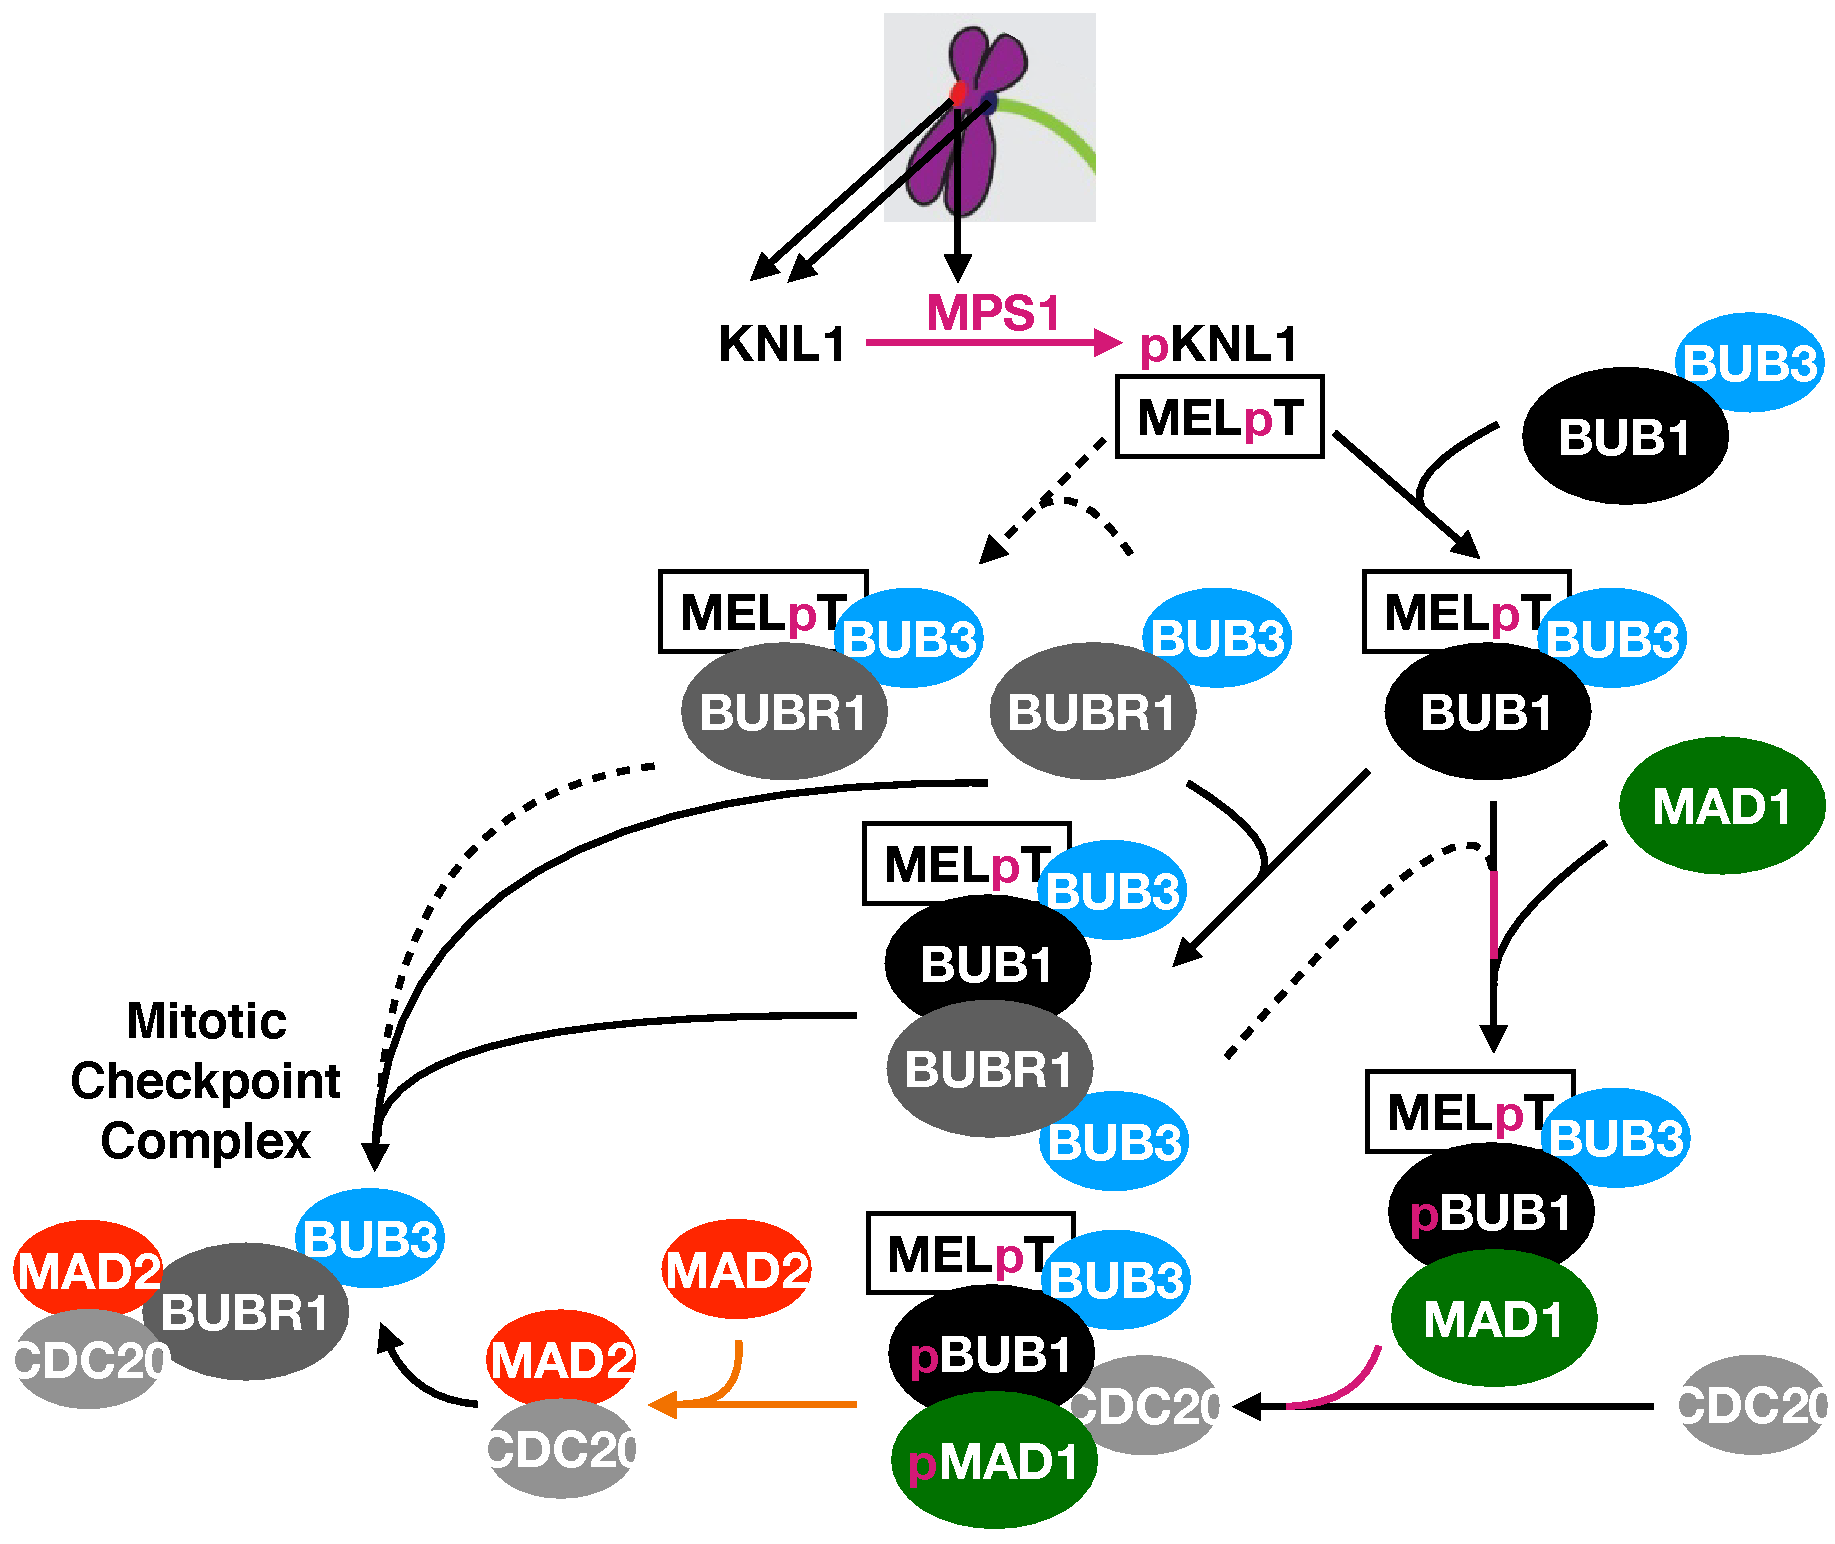
\includegraphics[width=\textwidth]{chapters/figures/CoreSAC.pdf}
    \caption{\textbf{The biochemical interactions and reactions of the core SAC signaling pathway.}}
    \noindent\justifying In the core SAC signaling pathway, signaling kinetochores recruit the kinase \protein{Mps1} which phosphorylates the consensus MELT motifs on the scaffold protein \protein{Knl1}. Phosphorylated MELT motifs (the ``MELpT'' rectangle in the figure) will then recruit a series of SAC proteins and eventually generate the effector molecule known as the Mitotic Checkpoint Complex (MCC), which blocks the progression of mitosis. Black solid arrows indicate direct binding or participation, which is either the consensus understanding \cite{MPS1Localization_Ji, MPS1Localization_Hiruma, RecombinantKNL1, MELTActivity, BubBiochem, BubR1TwoPools, BUB1CD1-MAD1CStructure, Faesen2017, BUB1-CDC20-MAD1, Tripartite} or experimentally proved in \myref{per_se}. Black dashed arrows indicate arguable \cite{BubBiochem, BubR1TwoPools} or hypothetical direct binding or participation. Magenta arrows and texts indicate \protein{Mps1} or the involvement of \protein{Mps1}-mediated phosphorylation \cite{Ji2017eLife}. The orange arrow indicate catalytic reactions leading to the formation of the \protein{Cdc20}-\protein{Mad2} dimer, which will be the focus of \myref{chpt:4}. The green \protein{Mad1} oval indicates the \protein{Mad1}-\protein{Mad2} heterotetramer (see \myref{chpt:4}). This heterotetramer is extremely stable in the budding yeast \cite{StableHeterotetramer}. The molecular weight of \protein{Mad1} (an extended protein mainly composed of \textalpha{}-helices according to the prediction of AlphaFold \cite{AlphaFold}) is also much larger than the molecular weight of \protein{Mad2} (a globular protein \cite{Structure1GO4}). Therefore, the \protein{Mad1}-\protein{Mad2} heterotetramer is also sometimes simply referred to as ``\protein{Mad1}'' in the following context.
    \label{CoreSAC}
\end{figure}

\protein{Knl1} possesses multiple consensus MELT motifs \cite{MELTEvolution}, which are phosphorylated at signaling kinetochores \cite{MPS1-KNL1_London2012, MPS1-KNL1_Shepperd2012, MPS1-KNL1_Yamagishi2012, MPS1Localization_Ji, MPS1Localization_Hiruma}. Phosphorylated MELT motifs initiate the core SAC signaling pathway by recruiting SAC proteins like \protein{Bub3}, \protein{Bub1}, \protein{BubR1}, \protein{Cdc20}, and the \protein{Mad1}-\protein{Mad2} heterotetramer, thereby promoting the assembly of the mitotic checkpoint complex (MCC) consisting of \protein{BubR1}/\protein{BubR1}-\protein{Bub3} and \protein{Cdc20}-\protein{Mad2} \cite{RecombinantKNL1, MELTActivity, BubBiochem, BubR1TwoPools, BUB1CD1-MAD1CStructure, Faesen2017, BUB1-CDC20-MAD1, Tripartite, SpMCC}. The mitotic checkpoint complex inhibits the E3 ubiquitin ligase anaphase-promoting complex/cyclosome (APC/C). APC/C ubiquinates a key mitosis regulator Cyclin B1 for proteasome-mediated degradation \cite{SeparaseStructure}. By inhibiting the APC/C, the degradation of Cyclin B1 is inhibited and the onset of anaphase is delayed.

In the corona pathway of the SAC signaling, the corona recruits the \protein{Mad1}-\protein{Mad2} heterotetramer to signaling kinetochores and promotes the SAC signaling activity. It should be noted that the core pathway and the corona pathway are not independent in human cells. It has been suggested that the recruitment of \protein{Mad1} to signaling kinetochores may be cooperative, facilitated by both RZZS and \protein{Bub1} \cite{MIS12-CEP57-MAD1-MAD2, siROD_Zhang2019}. \protein{Cdc20} also binds to signaling kinetochores cooperatively, faciliated by \protein{Bub1} and \protein{Mad1} \cite{BUB1-CDC20-MAD1, Tripartite}. We conceptually separate the two pathways because the corona does not exist in the budding yeast but the core pathway is conserved from yeast to human \cite{YeastNoRZZ}.

The \protein{Knl1} and the corona machinery also contribute to mitotic progression by facilitating chromosome congression. \protein{Knl1}-recruited \protein{BubR1} binds to the phosphatase \protein{PP2A-B56}, which stabilizes the kinetochore-microtubule attachment. The corona recruits the centromere-associated kinesin \protein{Cenp-E}, which promotes end-on attachment to spindle microtubules. The corona also promotes microtubule capture. Corona constituents \protein{Cenp-E} and \protein{Cenp-F} interact with \protein{BubR1} and \protein{Bub1}, respectively \cite{CENPELocalization-BUBR1, CENP-FLimitsStripping}.